\chapter{Oscillations and Waves}

\textbf{Periodic Motion} is a motion that regularly returns a certain position after fixed time.
\textbf{Simple Harmonic Motion} is a special kind of periodic motion where the magnitude of the 
net force acting on an object is proportional to the position of said object and its direction
opposite of the displacement of said object relative to its equilibrium position.

\section{Motion of an Object Attached to a Spring}

Consider the following system.

\begin{center}
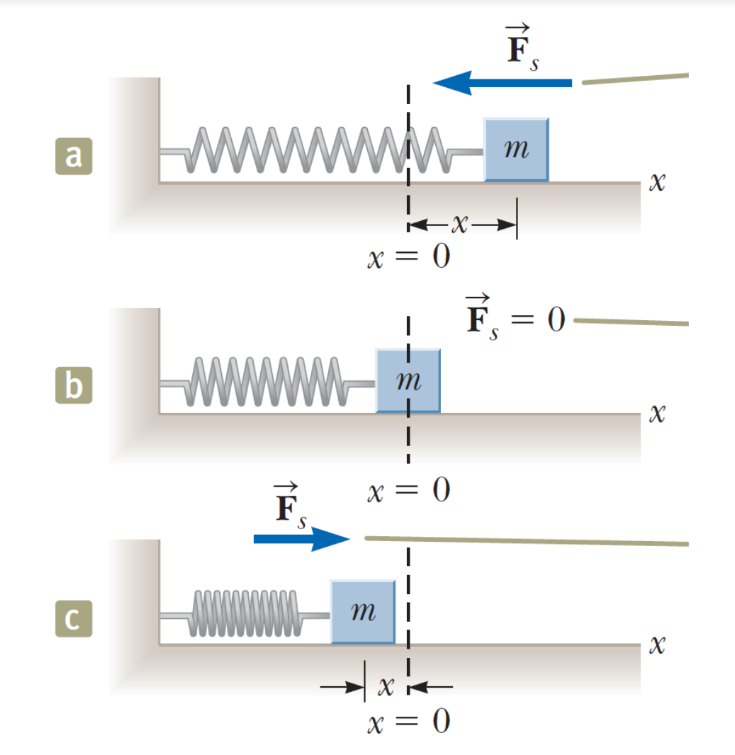
\includegraphics[scale=0.5]{oaw/spring01.png}\label{fig15.1}
\end{center}

When the spring is neither stretched or compressed, the block is at the \textbf{equilibirum position},
denoting as $x = 0$. When force is applied, the position of the block will move back and forth in an 
oscillating motion. We can model this using Hooke's law.

\begin{equation}\label{15.1}
    F_s = -kx
\end{equation} 

Here, we call $F_s$ the \textbf{restoring force} as it is always directed towards the equilibrium position.
Thus, it will always be opposite of the displacement of the block. Since there is some net force
acting on the object, even when released, we can apply Newton's second law of motion onto~\eqref{15.1}
to obtain

\begin{equation*}
    \sum F_x = ma_x \rightarrow -kx = ma_x
\end{equation*}

\begin{equation}\label{15.2}
    a_x = - \frac{k}{m}x
\end{equation}

This shows that the force applied on the object is proportional to $x$ and direction is opposite 
of the displacement. This is an example of a simple harmonic motion.

An example of how an object moves $-$ given the object starts at displacement $x=A$ and $x=0$ is the
equilibrium position:
\begin{itemize}
    \item Once released from rest, initial acceleration $a_i = -kA/m$ and speed is 0
    \item Once block is at $x=0$, acceleration is also zero and speed is at maximum
    \item Passing $x=0$, it moves with positive acceleration until $x=-A$, $a = +kA/m$, and speed is 0
    \item Moves back and passes $x=0$ again with maximum speed
\end{itemize}

In conclusion, the object oscillates between $x \in [-A, A]$. Note that we are consider this system
in the absence of friction. However, real-world systems are not frictionless, so please do keep that in mind.

\section{Analysis Model: Particle in Simple Harmonic Motion}

Recall equation from~\eqref{15.2}, we can turn $a$ into $d^2x / dt^2$ since accerelation is just
the second derivative of displacement and express it as
\begin{equation}\label{15.3}
-kx = ma_x = m\frac{d^2x}{dt^2} \implies \frac{d^2x}{dt^2} = -\frac{k}{m}x
\end{equation}

We can then express $k/m$ as $\omega^2$ then we can rewrite~\eqref{15.3} as 
\begin{equation}\label{15.5}
    \frac{d^2x}{dt^2} = - \omega^2 x
\end{equation}

We now arrive at a differential equation that we need to solve. In essence, we are trying to 
find a function $x$ whose second-order derivative is the same as the original with a negative sign.
We have a few choices: polynomic with negative power, exponential, logarithmic, and trigonometric
functions. Our choice? \textit{Trigonometric functions}, specifically $\sin$ and $\cos$. Finally,
we have found a suitable function $x$.
\begin{equation}\label{15.6}
    x(t) = A\sin(\omega t + \phi)
\end{equation} 
where $A$, $\omega$, and $\phi$ are constant parameters of the motion. Then, we can plot $x$ as
a function of $t$. These parameters (and some more) will then represent the following:
\begin{itemize}
    \item $A$ represents the \textbf{amplitude} $-$ the maximum value of position or $|x|\leq A$
    \item $\omega$ represents the \textbf{angular frequency} $-$ measure of how rapidly the oscillations
        are occurring, where \begin{equation}\label{15.9}
            \omega = \sqrt{\frac{k}{m}}
        \end{equation}
    \item $\phi$ represents the \textbf{phase constant} or \textbf{initial phase angle} $-$
        determined by the position and velocity position and velocity of object at $t=0$, where
        if $x=A$ at $t=0$, $\phi = 0$
    \item Quantity $(\omega t + \phi)$ represents the \textbf{phase} of the motion and the value of
        $x(t)$ has the same value when the $\omega t$ increasees by $2\pi$ radians
    \item $T$ represents the \textbf{period}, the time interval for object to return to go through
        a full cycle of motion
\end{itemize}


\subsection{Interpretation}

We can interpret $\omega$ as the angular frequency which is $2\pi f = 2\pi / T$.
Knowing that $\omega = \sqrt{k/m}$, this means that for a given spring with a certain $k$ and mass $m$,
we cannot change the way that it oscillates. No matter how much we stretch, it's going to bounce with
that frequency. This is called the \textbf{Natural Frequency}. The only way to change is to change 
the value of $k$ and $m$.

Simple Harmonic Motion refers to a motion with a single frequency $-$ $\omega$.
Obviously, there exists Harmonic Motion that are not simple. However, it is out of the scope of this course.

\subsection{Equation of Motion on a Pendulum}

\begin{center}
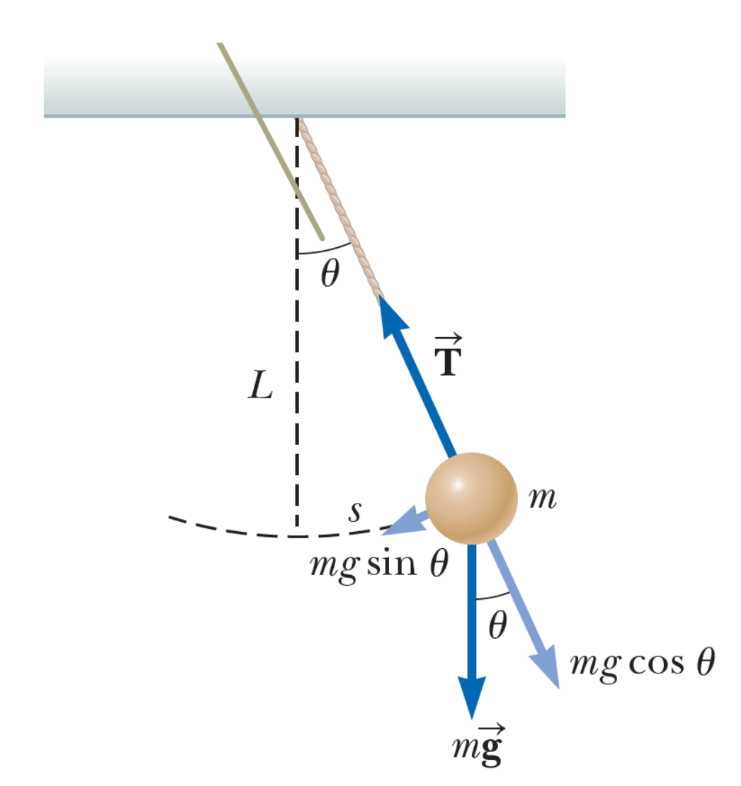
\includegraphics[scale=0.3]{images/oaw/pendulum01.png}
\end{center}

In order to analyze the motion of the pendulum, we can break down said motion into the vertical and
horizontal components. We can say that the tension $T = mg\cos\theta$ then completely ignore the motion's
vertical component as they cancel out. Therefore, the only remaining forces will be
\[\sum F_t = ma_t \implies -mg\sin\theta = m\frac{d^2s}{dt^2}\]
where $s$ is the tangential distance (displacement in circular motion). Once we cancel everything
and rearrange it such that it looks like our previous differential equation, we will get
\[ \frac{d^2s}{dt^2} = -g\sin\theta \]

This is where we need to face the harshness of reality. We cannot solve this equation, not without
a computer. However, we can use some approximation tricks to help us.

If the angle $\theta$ of swing is small, $\sin\theta \approx \theta$. We can also change $s$ into 
something easier to deal with. Since we know that $\theta = s/L$ where $L$ is the radius, we can
express $s$ as $\theta L$. With some manipulation, our equation then becomes
\[ \frac{d^2(\theta)}{dt^2} \approx -\frac{g}{L}\theta \]

Therefore, the (approximate) solution to this equation of motion is
\[ \theta(t) = A\sin(\omega t + \delta), \omega = \sqrt{\frac{g}{L}} \]

In this case, mass does not even matter to the oscillation. The only things that matter are the 
gravitational accerelation ($g$) and the length of the string attached to your pendulum ($L$).
Interestingly, this was how people made clocks back in the day.

\subsection{Equation of Motion on Rotation}

\begin{center}
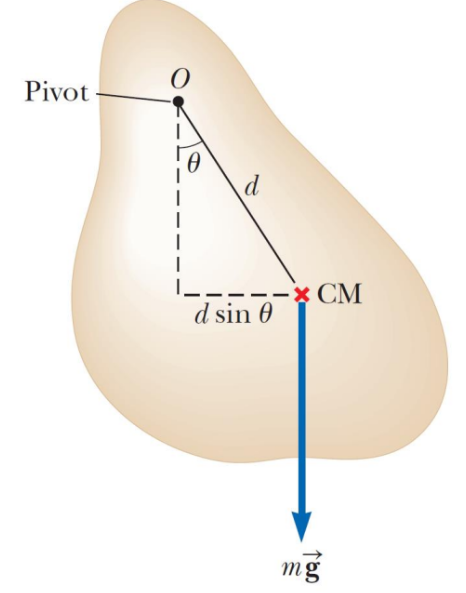
\includegraphics[scale=0.5]{images/oaw/rotation01.png}
\end{center}

Instead of Newton's equation, we now use $\vec{\tau} = I\vec{\alpha} = \vec{r}\times\vec{F}$.
From the diagram, we can see that the only thing generating torque is $m\vec{g}$. Let $r$ be the
distance from the pivot to the force (note that this distance is measured from $O$ to the point
perpendicular to the force), $r = d\sin\theta$. Now, torque will become $dmg\sin\theta$. Since
the torque is going clock-wise, the sign is negative. With some manipulation, our final 
approximate solution becomes
\[ \frac{d^2\theta}{dt^2} \approx -\frac{mgd}{I}\theta \]

Again, we can see that this is another simple harmonic motion where $\omega = \sqrt{(mgd)/I}$.

\subsection{Energy of Simple Harmonic Oscillator}

We can first find the kinetic and potential energy by
\begin{align*}
    K &= \frac{1}{2}mv^2 = \frac{1}{2}m\omega^2A^2\sin^2(\omega t + \phi)\\
    U &= \frac{1}{2}kx^2 = \frac{1}{2}A^2\cos^2(\omega t + \phi)
\end{align*}

Then, we can derive the total energy by
\begin{align*}
    E &= K + U\\
    &= \frac{1}{2}m\omega^2A^2\sin^2(\omega t + \phi) + \frac{1}{2}A^2\cos^2(\omega t + \phi)\\
    &= \frac{1}{2}kA^2 ( \sin^2(\omega t + phi) + \cos^2(\omega t + phi))\\
    &= \frac{1}{2}kA^2
\end{align*}
Note that since $\omega^2 \ k / m$, $(1/2)m(k/m) = (1/2)k$.

What does this mean? At any moment in time, the sum of the energy of the system must remain the same.
This aligns with the conservation of energy.